% Build:  cd presentation && tectonic main.tex
% (needs the `nanopulldown-presentation` conda env — see ../envs/presentation.yaml)
\documentclass[aspectratio=169]{beamer}

\usetheme{default}
\usepackage[utf8]{inputenc}
\usepackage{tikz}
\usetikzlibrary{arrows.meta, positioning, fit}
\usepackage{booktabs}
\usepackage[round]{natbib}
\usepackage{bibentry}
\nobibliography{refs}
\bibliographystyle{plainnat}
% centered (horizontally + vertically) multi-line table cell, no array.sty needed
\newcommand{\cc}[1]{\begin{tabular}[c]{@{}c@{}}#1\end{tabular}}
\usepackage{graphicx}
\setbeamerfont{footnote}{size=\tiny}
\setbeamercolor{footnote}{fg=muted}
% author-year style footnotes: no number, muted tiny text
\setbeamertemplate{footnote mark}{}
\renewcommand{\thefootnote}{}
\setbeamertemplate{footnote}{%
  \parindent 0em\noindent\raggedright
  {\usebeamercolor[fg]{footnote}\insertfootnotetext}\par}
\graphicspath{{figures/}{figures/logos/}{figures/license/}}

% --- Dark palette: navy / warm-white -------------------------------------
% Same high-contrast palette as the sibling ab_initio_pipeline deck
% (WCAG-checked: projector-safe against the navy background).
%   bg vs fg (body text):    16.95:1 (AAA)
%   bg vs accent (bullets):   5.79:1 (AA)
%   bg vs muted (footline):   7.16:1 (AAA)
%   bg vs substrate (emph):   7.46:1 (AAA)
\definecolor{bgdark}{HTML}{05171F}
\definecolor{fgtext}{HTML}{FDF6E3}
\definecolor{accent}{HTML}{2AA198}   % structure/links/bullets
\definecolor{muted}{HTML}{8FA6AD}    % footline / secondary text
\definecolor{substrate}{HTML}{A29CF2} % this deck's "key takeaway" highlight color

\setbeamertemplate{navigation symbols}{}
\setbeamercolor{background canvas}{bg=bgdark}
\setbeamercolor{normal text}{fg=fgtext, bg=bgdark}
\setbeamercolor{structure}{fg=accent}
\setbeamercolor{title}{fg=fgtext}
\setbeamercolor{subtitle}{fg=muted}
\setbeamercolor{author}{fg=muted}
\setbeamercolor{institute}{fg=muted}
\setbeamercolor{date}{fg=muted}
\setbeamercolor{frametitle}{fg=fgtext, bg=bgdark}
\setbeamercolor{itemize item}{fg=accent}
\setbeamercolor{itemize subitem}{fg=accent}
\setbeamercolor{enumerate item}{fg=accent}
\setbeamertemplate{itemize item}[circle]
\setbeamertemplate{itemize subitem}[circle]
\setbeamercolor{section in toc}{fg=fgtext}
\setbeamercolor{page number in head/foot}{fg=muted}
\setbeamerfont{frametitle}{series=\bfseries}

% --- header: section progress, no per-slide dots -------------------------
\setbeamercolor{section in head/foot}{fg=bgdark, bg=accent}
\setbeamerfont{section in head/foot}{size=\tiny}
\setbeamertemplate{headline}{%
  \begin{beamercolorbox}[wd=\paperwidth, ht=2.5ex, dp=0.9ex]{section in head/foot}
    \usebeamerfont{section in head/foot}\insertsectionnavigationhorizontal{\paperwidth}{}{}
  \end{beamercolorbox}%
}

% --- current subsection name, tracked by hand ----------------------------
\newcommand{\currentsubsectionname}{}
\newcommand{\emptysubsectionname}{}
\let\origsubsection\subsection
\renewcommand{\subsection}[1]{\origsubsection{#1}\gdef\currentsubsectionname{#1}}

\setbeamertemplate{frametitle}{%
  \nointerlineskip
  \begin{beamercolorbox}[wd=\paperwidth, sep=0.3cm]{frametitle}
    \usebeamerfont{frametitle}\insertframetitle\hfill
    \ifx\currentsubsectionname\emptysubsectionname\else
      {\normalfont\footnotesize\color{muted}\currentsubsectionname}%
    \fi
    \strut
  \end{beamercolorbox}%
}
% --- section-divider frame: big centered section name --------------------
\newcommand{\sectiondivider}[1]{%
  {\setbeamertemplate{frametitle}{}%
  \begin{frame}
    \vfill
    \begin{center}
      {\color{accent}\rule{0.35\textwidth}{0.6pt}}\\[1.1em]
      {\color{fgtext}\Huge\bfseries #1}\\[1.1em]
      {\color{accent}\rule{0.35\textwidth}{0.6pt}}
    \end{center}
    \vfill
  \end{frame}}%
}

\setbeamercolor{footlineright}{fg=muted, bg=bgdark}
\setbeamertemplate{footline}{%
  \leavevmode%
  \hbox{%
    \begin{beamercolorbox}[wd=\paperwidth, ht=2.6ex, dp=1.2ex, right, rightskip=0.3cm]{footlineright}
      \usebeamerfont{footline}\tiny CC BY 4.0~\raisebox{-0.15em}{
\includegraphics[height=1.4ex]{by-4.0-88x31.pdf}}\hspace{0.4em}\insertframenumber\,/\,\inserttotalframenumber
    \end{beamercolorbox}%
  }%
}
\makeatletter
\AtBeginDocument{%
  \g@addto@macro{\@listi}{\setlength{\itemsep}{0.5em}\setlength{\topsep}{0.5em}}
  \g@addto@macro{\@listii}{\setlength{\itemsep}{0.5em}\setlength{\topsep}{0.5em}}
}
\makeatother
\setbeamertemplate{sections/subsections in toc}[sections numbered]

\title{NanoPulldown: a Local \textit{In Silico} Pulldown Screen}
\subtitle{AlphaPulldown-style bait/prey screening with ESMFold2-Fast on a single Apple Silicon Mac Studio}
\author{Etienne Reboul}
\institute{Groupe Gibbérellines et adaptation à l'environnement\\
Institut de Biologie Moléculaire des Plantes (IBMP), Strasbourg}
\date{\today}

\begin{document}

{\setbeamercolor{blank head}{bg=bgdark}
\setbeamertemplate{headline}{%
  \begin{beamercolorbox}[wd=\paperwidth, ht=2.5ex, dp=0.9ex]{blank head}\end{beamercolorbox}%
}
\begin{frame}
  \begin{tikzpicture}[remember picture, overlay]
    \node[anchor=north] at ([yshift=-0.5cm]current page.north) {
      
\includegraphics[height=0.8cm]{cnrs-white.png}%
      \hspace{1.4cm}%
      {\setlength{\fboxsep}{4pt}\colorbox{white}{
\includegraphics[height=0.7cm]{ibmp-color.png}}}%
      \hspace{1.4cm}%
      
\includegraphics[height=0.8cm]{anr-white.png}
    };
  \end{tikzpicture}
  \titlepage
\end{frame}

\begin{frame}{Outline}
  \footnotesize
  \begin{columns}[t]
    \begin{column}{0.48\textwidth}
      \tableofcontents[sections={1,2,3}]
    \end{column}
    \begin{column}{0.48\textwidth}
      \tableofcontents[sections={4,5,6}]
    \end{column}
  \end{columns}
\end{frame}
}

% ---------------------------------------------------------------------
\section{Introduction}
% ---------------------------------------------------------------------
\gdef\currentsubsectionname{}
\sectiondivider{Introduction}

% ---- Part 1: pull-down background -----------------------------------------
\subsection{Background}

\begin{frame}{Pull-down assay: finding what binds a bait}
  \begin{columns}[c]
    \begin{column}{0.56\textwidth}
      \centering
      {\setlength{\fboxsep}{3pt}\colorbox{white}{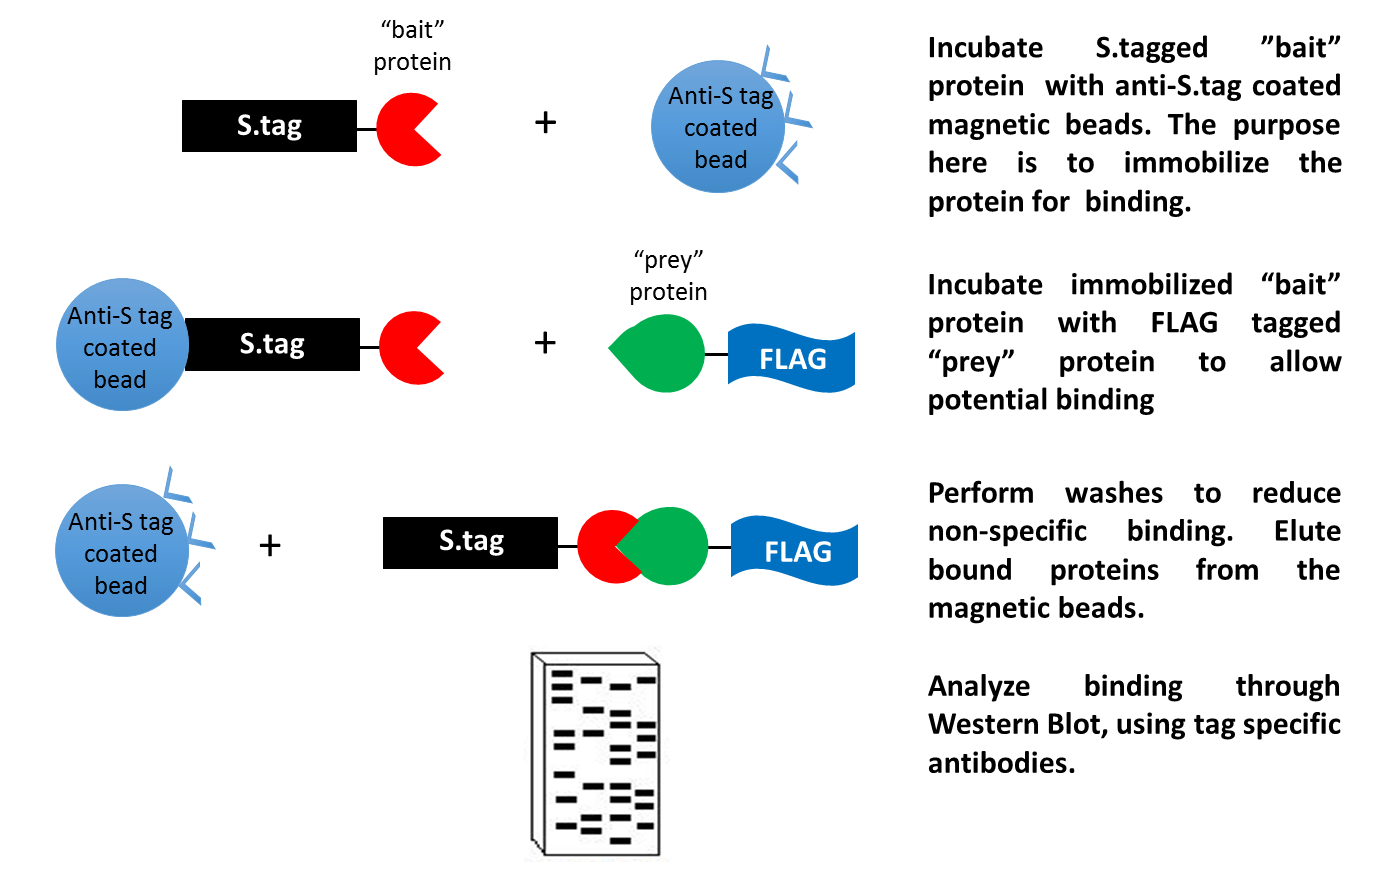
\includegraphics[width=\textwidth]{pulldown.png}}}\\[0.2em]
      {\tiny\color{muted} Pull-down with tagged proteins (S-tag / FLAG).
      RaihaT, Wikimedia Commons, CC BY-SA 3.0}
    \end{column}
    \begin{column}{0.42\textwidth}
      \begin{enumerate}
        \item \textbf{Pull-down}: tagged \emph{bait} immobilized on
          beads
        \item Incubate with \emph{prey} proteins (purified, or a lysate)
        \item Wash, then elute
        \item Readout: Western blot, or \textbf{mass spectrometry}
          (IP-MS) for a proteome-wide list of candidate preys
      \end{enumerate}
      \vspace{0.3em}
      \footnotesize
      \textcolor{substrate}{\textbf{Limits}}: direct and indirect binders are mixed.
    \end{column}
  \end{columns}
\end{frame}


\begin{frame}{The AlphaFold2 breakthrough}
  \centering
  {\setlength{\fboxsep}{2pt}\colorbox{white}{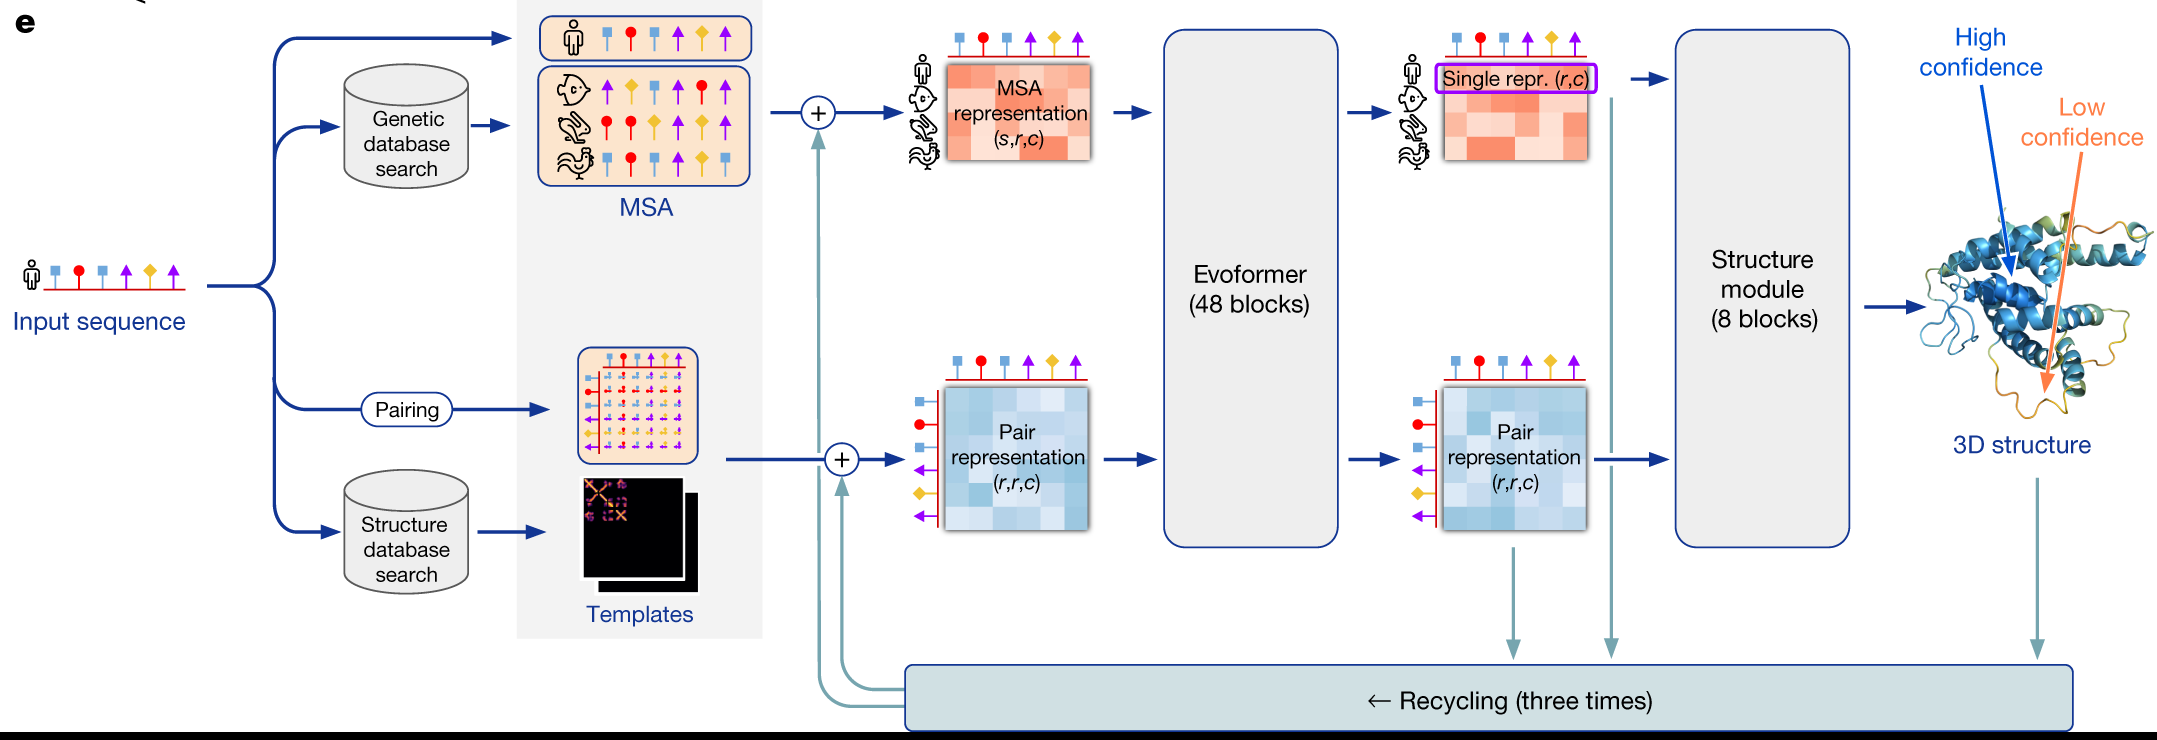
\includegraphics[width=0.93\textwidth]{af2_pipeline.png}}}\\[0.2em]
  {\tiny\color{muted} Fig.~1e, cropped; Wikimedia Commons, CC BY 4.0 \citep{jumper2021}\footnote{\bibentry{jumper2021}}}

  \vspace{0.3em}
  { 
  $\Rightarrow$ AF2 multimer is a \textbf{protein-protein docking engine} 
  with confidence scores}
\end{frame}

\begin{frame}{AlphaPulldown: the workflow}
  \centering
  {\setlength{\fboxsep}{3pt}\colorbox{white}{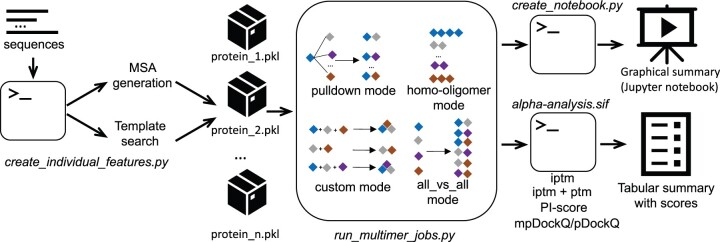
\includegraphics[width=0.78\textwidth]{alphapulldown.jpg}}}\\[0.2em]
  {\tiny\color{muted} Fig.~1 of the paper; CC BY 4.0 \citep{yu2023}\footnote{\bibentry{yu2023}}}

    \vspace{0.3em}
  { 
  $\Rightarrow$ AlphaPulldown automates identification of direct binding partners through the \textbf{in silico pulldown} with AF2-Multimer
  }
\end{frame}

% ---- Part 2: Problem statement ------------------------------------------------
\subsection{Problem statement}

\begin{frame}{Problem statement}
  \begin{itemize}
    \item AlphaPulldown is \textbf{great}, but it assumes:
      \begin{itemize}
        \item access to a GPU cluster : 
        \begin{itemize}
          \item Unmanageable to give access to a large number of users
          \item Pangloss (ibmp cluster) does not have high-end GPUs for a full screen
          \item High-end GPUs are expensive (around 12k EUR) currently not available through public procurement
        \end{itemize}
        \item MSA building :
        \begin{itemize}
          \item Typically a slow process with Jackhmmer and HHblits
          \item Requires large sequence databases (UniRef90, MGnify, BFD, PDB70, etc.)
          \item Not feasible on a laptop
        \end{itemize}
        \item AlphaFold models as docking engine :
        \begin{itemize}
          \item  AF2 multimer is no longer State-of-the-Art (SOTA) for protein-protein docking
          \item  AF3 weights are available on demand but have specific licensing restrictions
        \end{itemize}
      \end{itemize}
    \item[$\Rightarrow$] Can we run the same screen on a single MacStudio (range price : 3k-9k EUR)?
  \end{itemize}
\end{frame}

% ---- Part 3: language-model folding ---------------------------------------
\subsection{Language-model folding}

\begin{frame}{Protein LM as alternative folding engines}
  \normalsize
  \centering
  {\small Protein LMs (e.g.\ ESMFold, \citealp{lin2023}\footnote{\bibentry{lin2023}}):
  \textbf{LLM-style transformers} trained on proteins.}

  \vspace{0.8em}
  \renewcommand{\arraystretch}{1.15}
  \begin{tabular}{@{\hspace{0.6em}}c|c|c@{\hspace{0.6em}}}
    \toprule
     & \cc{\textbf{AF2-Multimer}} & \cc{\textbf{ESMFold-type (protein LM)}} \\
    \midrule
    \cc{Input} & \cc{sequence + \textbf{MSA} + templates}
      & \cc{\textbf{single sequence}} \\
    \midrule
    \cc{Evolutionary\\signal} & \cc{read from the alignment\\at inference}
      & \cc{\textbf{learned in the weights}\\during pre-training} \\
    \midrule
    \cc{Pre-processing} & \cc{database searches (slow, heavy)} & \cc{none} \\
    \midrule
    % Structure head & Evoformer + structure module & folding trunk on LM
    %   embeddings $\to$ structure module / diffusion \\
    \cc{Weak spot} & \cc{few homologs $\Rightarrow$ poor MSA}
      & \cc{orphan / novel sequences} \\
    \bottomrule
  \end{tabular}
\end{frame}

\begin{frame}{ESMFold2-Fast}
  \footnotesize
  \centering
  {\setlength{\fboxsep}{2pt}\colorbox{white}{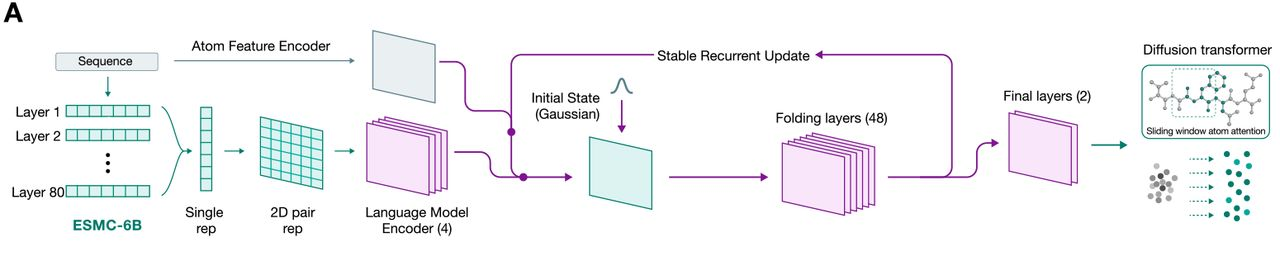
\includegraphics[width=0.85\textwidth]{esmfold2_arch.png}}}\\[0.1em]
  {\tiny\color{muted} Fig.~2A, cropped, CC BY 4.0 \citep{candido2026}\footnote{\bibentry{candido2026}}}

  \raggedright
  \begin{itemize}\scriptsize
    \item \textbf{ESMFold2-Fast} is designed for \textbf{high-throughput screening} and \textbf{design} of protein sequences
    \item \textbf{Simplified architecture}: 24 folding layers instead of 48 to reduce memory footprint and inference time
    \item \textbf{No MSA}: sequence-only prediction competitive with MSA-based methods (slightly worse than AF3)
    \item $\sim$9.4~s for 1\,024 residues on one H100 (reported 1.3$\times$
      faster than AF3)
    \item[$\Rightarrow$] \textcolor{substrate}{\textbf{This is what makes a
      high-throughput pulldown screen on a Mac Studio feasible}}
  \end{itemize}
\end{frame}

\subsection{Project Overview}
\begin{frame}{Motivation}
  \begin{itemize}
    \item A pulldown / IP-MS experiment returns a \textbf{long list} of
      candidate interactors -- which of them bind the bait \emph{directly}?
    \item Worked case: \textbf{BPM6} (AT3G43700, CUL3 substrate adaptor),
      GFP-IP in \textit{A.\ thaliana} (PXD013906, Chico \textit{et al.}\
      2020), 1 bait $\times$ $\sim$1\,500 prey candidates
    \item AlphaPulldown's UniProt-ID-driven bait/prey strategy answers
      this, but assumes AlphaFold-multimer/AF3, MSAs and a GPU cluster
    \item[$\Rightarrow$] Can we run the same screen \textbf{on one laptop}?
  \end{itemize}
\end{frame}

\begin{frame}{Design choices}
  \begin{enumerate}
    \item \textbf{ESMFold2-Fast} (MLX/Metal): no MSA, no templates, no
      cluster
    \item \textbf{Protein--protein only}: one seed, 1 diffusion sample per
      pair, no pose clustering
    \item \textbf{One command, one report}: a single Snakemake
      \texttt{rule all} from sequence annotation to the final report
    \item Adding pairs = a bait list + a prey list; pair specs are
      \textbf{generated}, not hand-written
  \end{enumerate}
\end{frame}

% ---------------------------------------------------------------------
\section{The pipeline}
% ---------------------------------------------------------------------
\gdef\currentsubsectionname{}
\sectiondivider{The pipeline}

\begin{frame}{Two stages, one diagram}
  \centering
  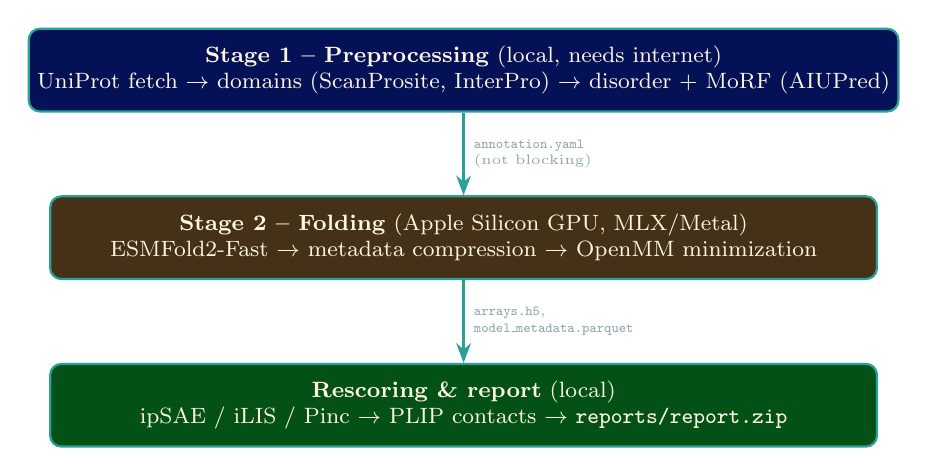
\begin{tikzpicture}[
      every node/.style={text=fgtext},
      stage/.style={draw=accent, thick, rounded corners, minimum width=10.5cm, minimum height=1.05cm,
                     align=center, font=\footnotesize, inner sep=3pt},
      arr/.style={-{Stealth[length=2.5mm]}, thick, draw=accent},
      lbl/.style={font=\tiny, text=muted, align=left}
    ]
    \node[stage, fill=blue!25!bgdark] (pre)  {\textbf{Stage 1 -- Preprocessing} (local, needs internet)\\
                                        UniProt fetch $\to$ domains (ScanProsite, InterPro) $\to$ disorder + MoRF (AIUPred)};
    \node[stage, fill=orange!25!bgdark, below=1.05cm of pre] (fold) {\textbf{Stage 2 -- Folding} (Apple Silicon GPU, MLX/Metal)\\
                                        ESMFold2-Fast $\to$ metadata compression $\to$ OpenMM minimization};
    \node[stage, fill=green!25!bgdark, below=1.05cm of fold] (post) {\textbf{Rescoring \& report} (local)\\
                                        ipSAE / iLIS / Pinc $\to$ PLIP contacts $\to$ \texttt{reports/report.zip}};
    \draw[arr] (pre) -- (fold) node[midway, right, lbl] {\texttt{annotation.yaml}\\(not blocking)};
    \draw[arr] (fold) -- (post) node[midway, right, lbl] {\texttt{arrays.h5},\\\texttt{model\_metadata.parquet}};
  \end{tikzpicture}

  \vspace{0.5em}
  {\footnotesize\textcolor{substrate}{\textbf{Everything runs on one machine, in one Snakemake call.}}}\par
\end{frame}

\begin{frame}{Stage 1 - Preprocessing}
  \begin{itemize}
    \item \textbf{Pair expansion}: \texttt{configs/baits.txt} $\times$
      \texttt{configs/preys.txt} (AlphaPulldown syntax:
      \texttt{ID}, \texttt{ID:N}, \texttt{ID:start-stop}) $\to$
      \texttt{configs/<bait>\_\_<prey>.yaml}; pairs over
      \texttt{esmfold2.max\_tokens} are skipped and listed
    \item \textbf{Domain annotation}: ScanProsite + InterPro API (fast
      path by accession; InterProScan v6 MATCH as fallback)
    \item \textbf{Disorder + MoRF}: AIUPred (docker), one container run per
      200 sequences
    \item Annotation runs \textbf{once per unique sequence} (cached) with
      polite, ramped rate limits on the public APIs
    \item[$\Rightarrow$] proposed \texttt{domains:} block, curated
      \textbf{whenever convenient} - it never blocks folding
  \end{itemize}
\end{frame}

\begin{frame}{Stage 2 : Folding}
  \begin{itemize}
    \item \textbf{ESMFold2-Fast} (\texttt{biohub/ESMFold2-Fast}), MLX on
      Metal: 10 loops, 100 sampling steps, 1 seed, 1 diffusion sample
    \item Memory-bound, not compute-bound: $\sim$25~GB model load in
      unified memory $\Rightarrow$ \texttt{--resources gpu=1} is
      \textbf{mandatory}
    \item \textbf{Batched folding}: 50 pairs per model load, so the model
      is loaded once per chunk, not once per pair
    \item \textbf{Token limit}: peak memory grows $\sim n^{2.2}$; measured
      on a 36~GB M4 Max, 1\,000 tokens $\approx$ 29~GB, 145~s
      (\texttt{max\_tokens: 1000})
    \item Metadata compression: pair ipTM / PAE $\to$ \texttt{arrays.h5} +
      \texttt{model\_metadata.parquet}
  \end{itemize}
\end{frame}

\begin{frame}{Minimization, rescoring and contacts}
  \begin{enumerate}
    \item \textbf{OpenMM minimization} (\texttt{amber14} + GBn2 implicit
      solvent; OpenCL with CPU fallback; divergence detection and failure
      table)
    \item \textbf{Rescoring}: ipSAE, iLIS, Pinc (PAE cutoff 12~\AA, C$\beta$
      contact cutoff 8~\AA) next to ESMFold2's own pair ipTM
    \item \textbf{PLIP} (docker, \texttt{linux/amd64} under Rosetta):
      bait $\leftrightarrow$ prey contacts per minimized sample, merged
      into \texttt{plip\_summary.csv} per pair
    \item PAE-based \textbf{domain $\times$ domain confidence heatmap} per
      sample
  \end{enumerate}
\end{frame}

\begin{frame}{Running it}
  \small
  {\ttfamily\scriptsize
  \begin{flushleft}
  conda env create -f envs/controller.yaml\\
  python scripts/expand\_pairs.py\ \ \ \ \# baits x preys -> configs/<pair>.yaml\\
  \# add the new pair stems to config.yaml's pairs: list\\
  snakemake --use-conda --cores 4 --resources gpu=1 docker\_heavy=3\\
  \end{flushleft}
  }
  \vspace{0.4em}
  \begin{itemize}
    \item \texttt{gpu=1}: caps \texttt{run\_esmfold2} at one model load --
      nothing else guards against concurrent loads (OOM)
    \item \texttt{docker\_heavy=N}: keeps minimization / PLIP containers
      from running during a model load, then lets $N$ run in parallel
    \item[$\Rightarrow$] \textcolor{substrate}{\textbf{Output: one
      \texttt{reports/report.zip}}}
  \end{itemize}
\end{frame}

% ---------------------------------------------------------------------
\section{Config and reuse}
% ---------------------------------------------------------------------
\gdef\currentsubsectionname{}
\sectiondivider{Config and reuse}

\begin{frame}{Adding a new screen}
  \small Edit \textbf{only}: the bait/prey lists, then one line per pair in
  \texttt{config.yaml}'s \texttt{pairs:}.
  \textcolor{substrate}{\textbf{No script edits.}}

  \vspace{0.6em}
  \begin{center}
  \footnotesize
  \begin{tabular}{@{}ll@{}}
    \toprule
    file & role \\
    \midrule
    \texttt{config.yaml} & shared defaults, both stages \\
    \texttt{config.local.yaml} & per-machine overrides (gitignored): InterPro e-mail, \texttt{max\_tokens} \\
    \texttt{configs/baits.txt}, \texttt{preys.txt} & one protein spec per line \\
    \texttt{configs/<bait>\_\_<prey>.yaml} & chain spec + curated domains (generated) \\
    \texttt{envs/} & one conda env per rule group (\texttt{--use-conda}) \\
    \bottomrule
  \end{tabular}
  \end{center}
\end{frame}

\begin{frame}{Reused from \texttt{ab\_initio\_pipeline}}
  \begin{itemize}
    \item Vendored \textbf{ipSAE} and \textbf{Pinc} (\texttt{tools/}),
      unchanged
    \item Same dark \texttt{custom.css} report theme and \texttt{datavzrd}
      tables
    \item Same annotation logic (domains, disorder), adapted:
      AIUPred replaces IUPred3/ANCHOR2 \textbf{and} MoRFchibi2 in one step
    \item \textbf{Replaced}: no HPC scheduler, no ABCfold backends, no MSA,
      no ChimeraX / antechamber (OpenMM instead), no pose clustering
  \end{itemize}
\end{frame}

% ---------------------------------------------------------------------
\section{Report}
% ---------------------------------------------------------------------
\gdef\currentsubsectionname{}
\sectiondivider{Report}

\begin{frame}{One report, zipped}
  \begin{itemize}
    \item Snakemake report, \textbf{SVG/PDF figures only}, dark theme
      (\texttt{report/custom.css})
    \item \textbf{Zip, not bare \texttt{.html}}: browsers block the
      \texttt{data:} URLs needed to embed interactive \texttt{datavzrd}
      tables $\to$ unzip, open \texttt{report.html}
    \item Contents:
      \begin{itemize}
        \item results table across all pairs (ipSAE / iLIS / Pinc / pair ipTM)
        \item PLIP contact heatmaps, domain-aware
        \item PAE domain $\times$ domain confidence heatmaps
        \item minimization energy plots + failure table
      \end{itemize}
    \item Stage-1 figures (domain map, disorder / binding) are kept as
      plain SVGs under \texttt{data/annotation/<pair>/}
  \end{itemize}
\end{frame}

% ---------------------------------------------------------------------
\section{Caveats and next steps}
% ---------------------------------------------------------------------
\gdef\currentsubsectionname{}
\sectiondivider{Caveats and next steps}

\begin{frame}{Assumptions still to confirm}
  \begin{itemize}
    \item \textbf{MLX path}: assumed to fill \texttt{result.pae} /
      \texttt{pair\_chains\_iptm} like the Torch/CUDA path to check
      against a live run
    \item \textbf{AIUPred CLI} (\texttt{-i/-t/-o}) and the \textbf{InterProScan
      v6 MATCH} endpoint: to confirm against current docs
    \item \textbf{OpenMM OpenCL} on Metal: CPU fallback exists, but
      initialization is untested on other Macs
    \item \textbf{PLIP on Apple Silicon}: amd64 emulation is slow and
      needs Rosetta in Docker Desktop
    \item \textbf{Memory}: 3 concurrent PLIP containers once caused a
      swap/OOM crash $\Rightarrow$ start with \texttt{docker\_heavy=2}
  \end{itemize}
\end{frame}

\begin{frame}{Roadmap}
  \begin{itemize}
    \item Complete the BPM6 screen over the PXD013906 prey list and compare
      ranking against the PNAS Dataset~S1 known / significant interactors
    \item Benchmark ESMFold2-Fast ranking metrics (ipSAE, iLIS, pair ipTM)
      on known positives vs.\ random preys
    \item Tune \texttt{max\_tokens} and \texttt{pairs\_per\_load} per machine
      (\texttt{notebooks/esmfold2\_memory\_model.ipynb})
    \item Optional: re-fold top hits with AF3 / ABCfold for confirmation
  \end{itemize}
\end{frame}

\begin{frame}
  \centering
  \Huge Questions?
\end{frame}

% register citations for \citep (and run bibtex) without printing a reference list
\setbox0\vbox{\bibliography{refs}}

\end{document}
